% !TEX TS-program = pdflatex
% !TEX encoding = UTF-8 Unicode

% This is a simple template for a LaTeX document using the "article" class.
% See "book", "report", "letter" for other types of document.

\documentclass[11pt]{article} % use larger type; default would be 10pt

\usepackage[utf8]{inputenc} % set input encoding (not needed with XeLaTeX)

%%% Examples of Article customizations
% These packages are optional, depending whether you want the features they provide.
% See the LaTeX Companion or other references for full information.

%%% PAGE DIMENSIONS
\usepackage[a4paper, total={6in, 9in}]{geometry} % or letterpaper (US) or a5paper or....
% \geometry{margin=2in} % for example, change the margins to 2 inches all round
% \geometry{landscape} % set up the page for landscape
%   read geometry.pdf for detailed page layout information

\usepackage{graphicx} % support the \includegraphics command and options

% \usepackage[parfill]{parskip} % Activate to begin paragraphs with an empty line rather than an indent

%%% PACKAGES
\usepackage{booktabs} % for much better looking tables
\usepackage{array} % for better arrays (eg matrices) in maths
\usepackage{paralist} % very flexible & customisable lists (eg. enumerate/itemize, etc.)
\usepackage{verbatim} % adds environment for commenting out blocks of text & for better verbatim
\usepackage{subfig} % make it possible to include more than one captioned figure/table in a single float
% These packages are all incorporated in the memoir class to one degree or another...
\usepackage{listings}
\usepackage{xcolor}
\usepackage{amsmath}
\usepackage{float}

\definecolor{codegreen}{rgb}{0,0.6,0}
\definecolor{codegray}{rgb}{0.5,0.5,0.5}
\definecolor{codepurple}{rgb}{0.58,0,0.82}
\definecolor{backcolour}{rgb}{0.95,0.95,0.92}

\lstdefinestyle{mystyle}{
    backgroundcolor=\color{backcolour},   
    commentstyle=\color{codegreen},
    keywordstyle=\color{magenta},
    numberstyle=\tiny\color{codegray},
    stringstyle=\color{codepurple},
    basicstyle=\ttfamily\footnotesize,
    breakatwhitespace=false,         
    breaklines=true,                 
    captionpos=b,                    
    keepspaces=true,                 
    numbers=left,                    
    numbersep=5pt,                  
    showspaces=false,                
    showstringspaces=false,
    showtabs=false,                  
    tabsize=2
}

\lstset{style=mystyle}


%%% HEADERS & FOOTERS
\usepackage{fancyhdr} % This should be set AFTER setting up the page geometry
\pagestyle{fancy} % options: empty , plain , fancy
\renewcommand{\headrulewidth}{0pt} % customise the layout...
\lhead{}\chead{}\rhead{}
\lfoot{}\cfoot{\thepage}\rfoot{}

%%% SECTION TITLE APPEARANCE
\usepackage{sectsty}
\allsectionsfont{\sffamily\mdseries\upshape} % (See the fntguide.pdf for font help)
% (This matches ConTeXt defaults)

%%% ToC (table of contents) APPEARANCE
\usepackage[nottoc,notlof,notlot]{tocbibind} % Put the bibliography in the ToC
\usepackage[titles,subfigure]{tocloft} % Alter the style of the Table of Contents
\renewcommand{\cftsecfont}{\rmfamily\mdseries\upshape}
\renewcommand{\cftsecpagefont}{\rmfamily\mdseries\upshape} % No bold!

%%% END Article customizations

%%% The "real" document content comes below...

\title{AE 342 : Modeling and Analysis Lab, Session 4}
\author{Gaurav Gupta, SC21B026, Aerospace Engineering}
%\date{} % Activate to display a given date or no date (if empty),
         % otherwise the current date is printed 

\begin{document}
\maketitle

\section{Problem 1}
A simple 1D heat diffusion problem with Dirichlet boundary conditions is simulated. The governing equations and boundary conditions are provided as follows

\begin{equation}
\frac{d^2u}{dx^2} = 1, 0 < x < 1 
\end{equation}

\begin{equation}
u(x=0) = 0 \text{,  } u(x=1) = 0 
\end{equation}

The problem is solved in FreeFEM++ using the given code for a 1D domain. 

\begin{lstlisting}[language=C++, caption=Problem 1 Code ]
load "msh3"
real m = 100;
int l=1;
meshL Th = segment(m,[x*l]);
real[int] xaxis(m+1), Uline(m+1);
ofstream file2("Results.csv");

fespace Vh(Th, P1);
Vh U, v;

solve Poission(U,v)= int1d(Th)(dx(U)*dx(v))
				+int1d(Th)(v)
				+on(1,2, U=0);

plot(U, value=true);
for(int i=0; i<=m; i++){
	
	xaxis[i] = i/m;
	Uline[i] = U[][i];
	file2 << xaxis[i] << "," << Uline[i] << endl ;
}
\end{lstlisting}

The analytical solution for the problem is given as $U = \frac{1}{2}(x^2 - x)$. The solution of FreeFEM is compared to the analytical solution, 

\begin{figure}[H]
\centering
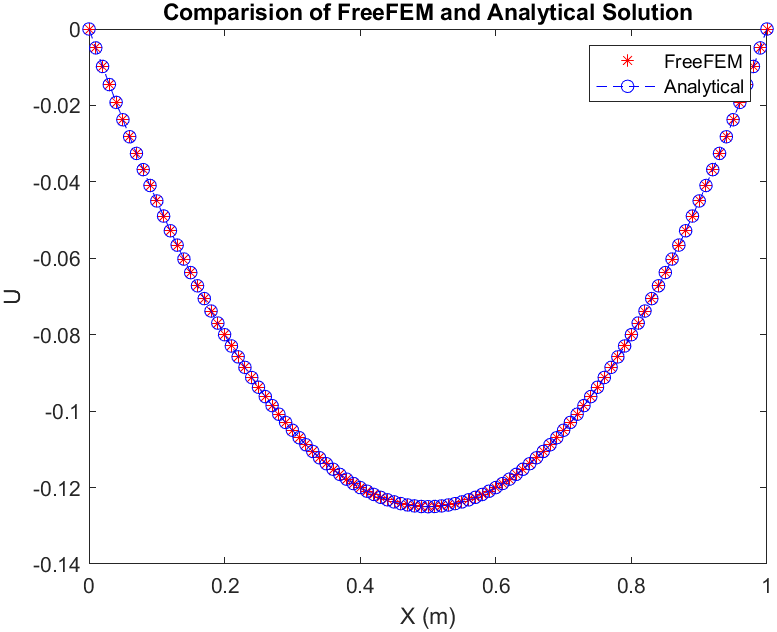
\includegraphics[width=0.85\textwidth]{q1.png}
\caption{Comparision of the FreeFEM Solution with analytical solution for Problem 1.}
\end{figure}

\section{Problem 2}
Consider a 1mm diameter, 50mm long aluminium pin-fin. The fin' s left end interfaces with a constant heat source at a temperature of $ T_{h} = 300^\circ C$, while its right end is thermally insulated. Heat is progressively released along the fin’s length through convection, interacting with an ambient temperature of $ T_{\infty} = 30^\circ C$. The governing differential equation is given by:

\begin{equation}\label{eqn:p2}
k\frac{d^2 T}{dx^2} = \frac{P h}{A}(T - T_{\infty}) 
\end{equation}

In equation \ref{eqn:p2}, the thermal conductivity (k) is 200 W/mK and the convective heat transfer coefficient (h) is $20W/m^2 K$. P, A represents perimeter and area of cross-section of the fin. Establish a model for the temperature distribution along the fin under these specific conditions and compare with analytical results.\\

The weak form of the equation \ref{eqn:p2} is given as 

\begin{equation}
\int_{\phi} \left( k \frac{dT}{dx} \frac{dv}{dx} + \frac{P h}{A}(T - T_{\infty}) \right) dx = 0
\end{equation}

\newpage
The problem is solved in FreeFEM++ using the given code for a 1D domain.
\begin{lstlisting}[language=C++, caption=Problem 2 Code ]
load "msh3"
real m = 100; 
real d = 0.001;
int h = 20;
int k = 200;
real l=0.05; 
int Ti = 300;
int Tf = 30;
real p = pi * d;
real A = pi * d * d / 4;

meshL Th = segment(m,[x*l]);

real[int] xaxis(m+1), Uline(m+1);
ofstream file2("results2.csv");

fespace Vh(Th, P1);
Vh T, v;

solve Poission(T,v)  = int1d(Th)(k*dx(T)*dx(v))
				+int1d(Th)(p*h/A*T*v)
				-int1d(Th)(p*h/A*Tf*v)
				+on(1, T=300);

plot(T, value=true, wait=true, fill=true, aspectratio=true);
for(int i=0; i<=m; i++){
	
	xaxis[i] = l * i/m;
	Uline[i] = T[][i];
	file2 << xaxis[i] << "," << Uline[i] << endl ;
}
\end{lstlisting}

The analytical solution for the problem is given as $T =  T_{\infty} + \left(\frac{270}{1+e^{2mL}}\right) \left(e^{mx} + e^{2ml -mx} \right)$. The solution of FreeFEM is compared to the analytical solution in Figure \ref{fig:q2}.\\

When the right end is subjected to the ambient temperature $ T_{\infty} = 30$ instead of the adiabatic condition. The analytical solution of the problem is given as $T =  T_{\infty} + \left(\frac{-270}{1-e^{2mL}}\right) \left(e^{mx} - e^{2ml -mx} \right)$. The result of this problem solved in FreeFEM is again compared to the analytical solution in Figure \ref{fig:q22}.\\

\vspace{0.5cm}

\begin{lstlisting}[language=C++, caption=Change in the Problem 2 Code to accomodate for the Dirchlet B.C. at the right end]
solve Poission(T,v)  = int1d(Th)(k*dx(T)*dx(v))
				+int1d(Th)(p*h/A*T*v)
				-int1d(Th)(p*h/A*Tf*v)
				+on(1,T=300)
				+on(2,T=30);
\end{lstlisting}

\begin{figure}[H]
\centering
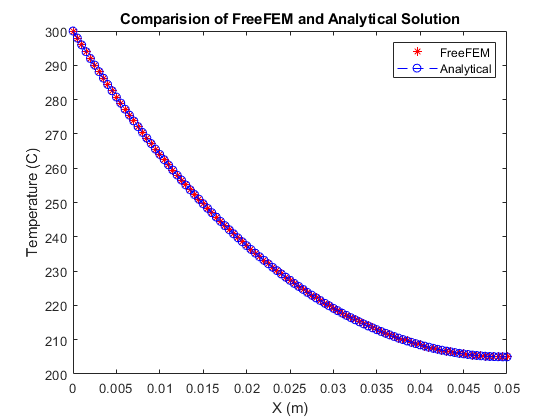
\includegraphics[width=0.75\textwidth]{q2.png}
\caption{Comparision of the FreeFEM Solution with analytical solution for Problem 2.}
\label{fig:q2}
\end{figure}

\begin{figure}[H]
\centering
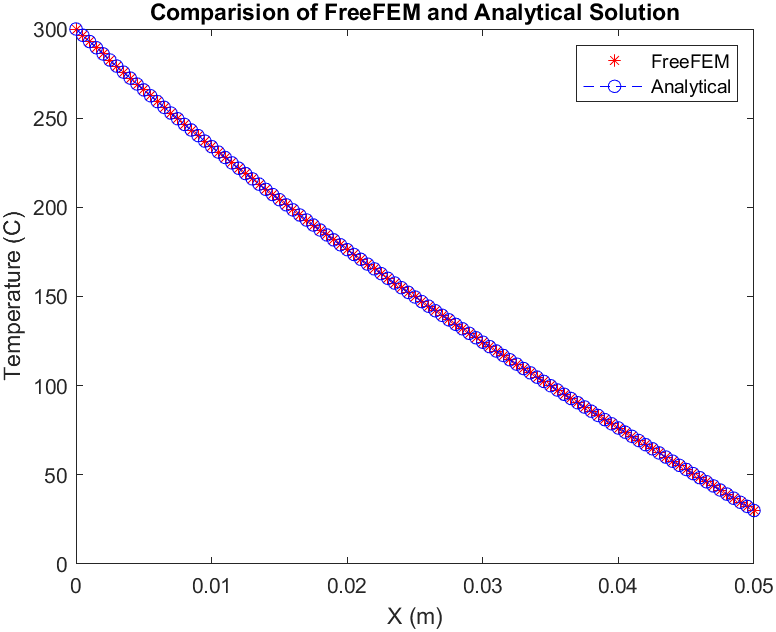
\includegraphics[width=0.7\textwidth]{q22.png}
\caption{Comparision of the FreeFEM Solution with analytical solution for Problem 2 with Dirchlet boundary condition at right end.}
\label{fig:q22}
\end{figure}

\newpage
\section{Problem 3}
Consider a rectangular plate of dimensions $L_x \times L_y$, where one side is insulated, while the other three sides are maintained at constant temperatures. The temperature distribution $T(x, y)$ in the plate is governed by Laplace’s equation:

\begin{equation}
 \nabla^2 T = 0
\end{equation}

\textbf{Boundary Conditions:}
\begin{itemize}
\item At $x = 0$: $\frac{\partial{T}}{\partial{x}}= 0$
\item At $x = L_x$ : $T(L_x, y) = 200^\circ C$
\item At $y = 0$ : $T(x, 0) = 150^\circ C$
\item At $y = L_y$ : $T(x, L_y) = 150^\circ C$
\end{itemize}

The weak formulation of the laplace equation is given as,
\begin{equation}
\int_{\phi} \left( \frac{dT}{dx} \frac{dv}{dx} +   \frac{dT}{dy} \frac{dv}{dy} \right) dx = 0
\end{equation}

\begin{lstlisting}[language=C++, caption=Code to solve  Problem 3 in FreeFEM]
load "msh3"

real Lx = 1;
real Ly = 2;
int m = 100;
int n = 200;
mesh Th=square(m,n,[Lx*x,Ly*y]);
//plot(Th, wait=true);
//real[int] V = [150, 155, 160, 165, 170, 175, 180, 185, 190, 195, 200];

fespace Vh(Th, P1);
Vh T, v;

solve Laplace(T,v) = int2d(Th)(dx(T)*dx(v) + dy(T)*dy(v))
				+on(1,3,T=150)
				+on(2,T=200);

plot(T, wait=true, fill=true, value=true, aspectratio=true);
\end{lstlisting}

The temperature distirbution $T(x,y)$ for the problem 3 is plotted in Figure \ref{fig:q3}.

\begin{figure}[H]
\centering
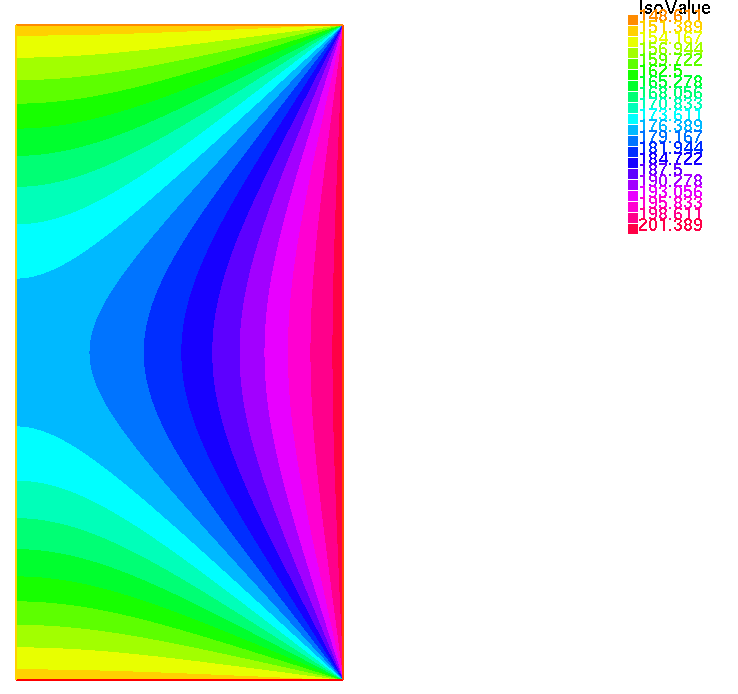
\includegraphics[width=0.75\textwidth]{q3.png}
\caption{temperature distirbution $T(x,y)$ for the problem 3 plotted in FreeFEM.}
\label{fig:q3}
\end{figure}

\end{document}

